\setcounter{page}{1}
\section*{Zielsetzung}
Im Versuch 18 \textit{Der Reinst-Germanium-Detektor als
Instrument der Gamma-Spektroskopie} sollen die theoretischen und experimentellen Grundlagen eines
Germaniumdetektors erarbeitet werden. Neben einer Einführung in die physikalischen Mechanismen der
Strahlungsabsorption in Festkörpern, wird im Folgenden die elektrische Beschaltung des Detektors beschrieben.
Die durchgeführten Messungen dienen der Kalibration des Detektors, sowie der Identifikation von unbekannten
Strahlungsquellen anhand aufgenommener Energiespektren.

\section{Theorie}
Die Detektion von Gamma-Strahlung in einem Germanium-Detektor basiert grundlegend auf der Tatsache, dass diese in dem
Detektormaterial an Intensität verliert. Durch Ionisationsprozesse werden freie Ladungsträger erzeugt, die letztlich
zu einem Spannungsimpuls führen, dessen Höhe Aufschluss über die Energie der einfallenden Photonen gibt.
Zunächst sollen an dieser Stelle die drei wichtigsten mikroskopischen Wechselwirkungseffekte zwischen Gamma-Srahlung und
Materie vorgestellt werden. Die eigentlichen Detektionsmechanismen lassen sich dann anschließend qualitativ im
Bändermodell für Festkörper beschreiben.

Eine wichtige physikalische
Größe zum Verständnis von Wechselwirkungsprozessen ist der Wirkungsquerschnitt $\sigma$ und sein Verhalten unter
Änderung der Energie $\frac{\mathup{d}\sigma}{\mathup{d}E}$ (differentieller Wirkungsquerschnitt). Der Wirkungsquerschnitt
ist ein Maß für die Wechselwirkungswahrscheinlichkeit und so lässt sich der Intensitätsverlust $\Delta I(D)$ von Strahlung beim Durchgang einer
Strecke $D$ im Festkörper formulieren zu
\begin{equation}
    \Delta I(D) = I_0 \left[1 -  \exp\left(- n \sigma D\right)\right].
\end{equation}
Hierin ist $n$ die Zahl der Elektronen pro Volumen. Das Produkt $\mu = n \sigma$ wird als Extinktionskoeffizient
bezeichnet und entspricht dem Kehrwert der mittleren Reichweite der Strahlung.

\subsection{Absorptionsmechanismen}
Als \textbf{Photoeffekt} bezeichnet man die Ionisierung eines Atoms durch ein einfallendes Photon. Im Fall der
hochenergetischen ($E_\gamma \geq  \SI{200}{\kilo\electronvolt}$) Gamma-Strahlung wird ein Elektron aus einer der stark gebundenen Schalen
ausgelöst. Hierbei verliert das Photon seine ganze Energie und die zurück bleibende Elektronenfehlstelle wird durch
höher liegende Elektronen unter Aussendung von charakteristischer Röntgenstrahlung aufgefüllt.
Für den Photoeffekt lässt sich zeigen, dass der Wirkungsquerschnitt $\sigma_{\text{Ph}}$ in Abhängigkeit der Energie und
Kernladungszahl $Z$ der beteiligten Atome annähernd zu beschreiben ist durch
\begin{equation}
    \sigma_{\text{Ph}} \sim Z^{\alpha} E^{\delta}, \quad 4 < \alpha < 5, \, \delta \approx -\num{3.5}.
    \label{eq:wirkungsquerschnitt_photo}
\end{equation}
Der Wirkungsquerschnitt des Photoeffekts nimmt also mit steigender Energie ab.

Eine zweite in diesem Versuch zu beobachtende Erscheinung ist der \textbf{Compton-Effekt}. Dieser lässt sich rein
klassisch als inelastischer Stoß eines Photons mit einem ruhenden, punktförmigen Elektron der äußeren Schalen verstehen.
Das Photon besitzt nach dem Stoß im Gegensatz zum Photoeffekt eine geringere Energie $E'_\gamma \neq 0$:
\begin{equation}
    {E'}_{\!\gamma} = \frac{E_\gamma}{1 + \frac{E_\gamma}{m_e c^2} \left(1 - \cos\vartheta \right)},
    \label{eq:rückstreu}
\end{equation}
mit dem Streuwinkel des Photons $\vartheta$. Der maximale Energieübertrag an das beteiligte Elektron findet für eine
Rückwärtsstreuung ($\vartheta = \pi$) statt. Der differentielle Wirkungsquerschnitt $\frac{\mathup{d}\sigma}{\mathup{d}E}$
(in Bezug auf die Elektronenenergie, die letztlich gemessen wird) verfügt also über einen kontinuierlichen Verlauf, der
bei einer maximalen Energie $E_{max} < E_\gamma$ (Compton-Kante) abbricht. Diese Elektronenenergie ist gegeben durch
\begin{equation}
    E_{max} = E_\gamma \frac{2\frac{E_\gamma}{m_ec^2}}{1 + 2\frac{E_\gamma}{m_ec^2}}
    \label{eq: comptonkante_energie}
\end{equation}
Das Ziel der Gamma-Spektrometrie ist es die
gesamte Energie des einfallenden Photons zu vermessen, da diese Rückschlüsse auf die atomare Struktur der Quelle
erlaubt. Der Compton-Effekt ist im Gegensatz zum Photo-Effekt daher eine eher störende Nebenerscheinung.
Der Wirkungsquerschnitt $\sigma{Co}$ lässt sich für kleine Energien $\varepsilon = E_\gamma / m c^2 << 1$
durch folgende Gleichung beschreiben
\begin{equation}
    \sigma_{Co} \sim \frac{3}{4}\sigma_{Th} \left(1 - 2\varepsilon + \frac{26}{5}\varepsilon^2 \right).
\end{equation}
Hierin ist $\sigma_{Th}$ der Thomsonsche Streuquerschnitt.

Der letzte hier diskutierte Effekt für die Gamma-Spektrometrie, der jedoch hier nicht beobachtet werden kann, ist die
\textbf{Paarerzeugung}. Ist die Energie des Photons größer als die zweifache Elektronenruheenergie $2m_ec^2$,
kann unter Beteiligung eines Atoms oder Elektrons ein Elektron-Positron-Paar erzeugt werden. Die Gesamtenergie
des Photons kann nur dann detektiert werden, wenn das Positron nicht rekombiniert. Die hierbei enstehenden
zwei Photonen können den Detektor verlassen, sodass insgesamt drei Peaks im Spektrum bei $E_\gamma$, $E_\gamma - m_ec^2$ (\emph{Single Escape Peak})
und $E_\gamma - 2m_ec^2$ (\emph{Double Escape Peak}) beobachtet werden.
Der Wirkungsquerschnitt $\sigma_{Pa}$ kann hier für zwei Grenzfälle angegeben werden: \\
Paarbldung in Kernnähe (kleine Abschirmung):
\begin{equation}
    \sigma_{Pa} \sim Z^2\left(\frac{28}{9} \mathup{ln}2\varepsilon - \frac{218}{27} \right).
\end{equation}
Paarbildung außerhalb der Elektronenhülle (starke Abschirmung):
\begin{equation}
    \sigma_{Pa} \sim Z^2 \left(\frac{28}{9}\mathup{ln}\frac{183}{Z^{\sfrac{1}{3}}} - \frac{2}{27} \right).
\end{equation}
Mit der Kernladungszahl $Z$. Eine grafische Zusammenfassung der verschiedenen
Absorptionsmechanismen befindet sich in Abbildung~\ref{fig:extinktionskoeffizient}. Hier ist der Extinktionskoeffizient
von Germanium als Funktion der Energie augetragen.


\subsection{Funktion des Germanium-Detektors}
Germanium ist ein indirekter Halbeiter mit einer minimalen Bandlückenenergie von ca. $\SI{0.6}{\electronvolt}$ am $L$-Punkt.
Die Absorption eines Photons lässt sich im Bändermodell durch das Anregen eines Elektrons aus dem Valenz- in das
Leitungsband verstehen. Bei diesem Prozess bleibt ein Loch im Valenzband zurück. Zentrales Element des Detektors ist nun
eine Anordnung aus einer $n$- und einer $p$-dotierten Germanium Schicht. An der Grenze zwischen den Schichten, wo Elektronen
und Löcher rekombinieren, bildet sich eine sogenannte Verarmungszone aus. Dieser Bereich ist zur Detektion von Strahlung
geeignet, da erzeugte Elektron-Loch-Paare durch das wirkende elektrische Feld voneinander getrennt werden können und somit ein
endlicher Stromfluss erzeugt wird. Durch das Anlegen einer äußeren Spannung kann die Verarmungszone vergrößert werden. Hierbei ist jedoch
zu beachten, dass für von $\SI{0}{\kelvin}$ verschiedene Temperaturen immer thermisch angeregte Ladungsträger im Leitungsband existieren, die
zu einem ständigen Stromfluss führen. Eine Erhöhung der Spannung muss daher immer mit einer Kühlung des
Halbleiterelements einher gehen. Eine weitere Methode zur Einstellung der Veramrungszone ist die Wahl des Dotierungverhältnisses.

Aufgabe der elektrischen Schaltung, die im nächsten Abschnitt besprochen wird, ist nun die am Germaniumdetektor erzeugten Spannungspulse der
Größe nach geordnet in Kanäle einzuordnen. Ein exemplarisches, so erzeugtes Energiespektrum befindet sich in
Abbildung~\ref{fig: example_spectrum}. Hier sind noch einmal die eingangs besprochenen Effekte zu erkennen. Zunächst besitzt jeder
Detektor eine untere Nachweisgrenze, die mindestens um die Bandlückenenergie vom Nullpunkt abweicht. Meist begrenzen jedoch
andere Gegebenheiten die Auflösung des Detektors, z.\,B. die Verkleidung des Detektors, die nur Photonen ab einer bestimmten Energie
durchdringen können. Weiter ist die kontinuierliche energetische Verteilung der Elektronen zu erkennen, die am Compton-Effekt
beteiligt waren (Compton-Kontinuum). Auch energetisch oberhalb der Compton-Kante werden noch einige wenige Spannungspulse gemessen,
was durch das Auftreten von mehrfachen Streuprozessen zu verstehen ist. Innerhalb des Compton-Kontinuums ist noch ein Rückstreupeak
zu erkennen. Dieser entsteht, wenn Photonen zunächst etwa an der Detektorwand Compton-gestreut werden und dann durch den
Photoeffekt ihre Energie an Elektronen im Detektor abgeben.
Die für die Spektrometrie eigentlich relevante Eigenschaft des Spektrums ist der Vollenergiepeak (oder die Vollenergiepeaks, falls
das Spektrum der Quelle mehrere Linien besitzt). An dieser Stelle werden Pulse gezählt, die durch Elektronen enstehen, welchen
die Gesamtenergie der Photonen übertragen wurde.
Seine Höhe und Position sind Merkmale, die quantitative Aussagen über die Strahlungsquelle ermöglichen.

%Es ist abschließend noch zu
%erwähnen, dass der Wirkungsquerschnitt des Photoeffekts für die hier betrachteten Energieskalen
%($E \sim \SI{1}{\mega\electronvolt}$) eigentlich kleiner ist als derjenige des Compton-Effekts. Dennoch ist der Gesamtenergiepeak
%höher als das Compton-Kontiunuum. Dies liegt daran, dass der Photowirkungsquerschnitt mit fallender Energie ansteigt
%und so Prozesse, bei denen vor dem Photoeffekt zunächst andere Streuungen stattfinden, ebenfalls in den Peak fallen können.

\begin{figure}
\centering
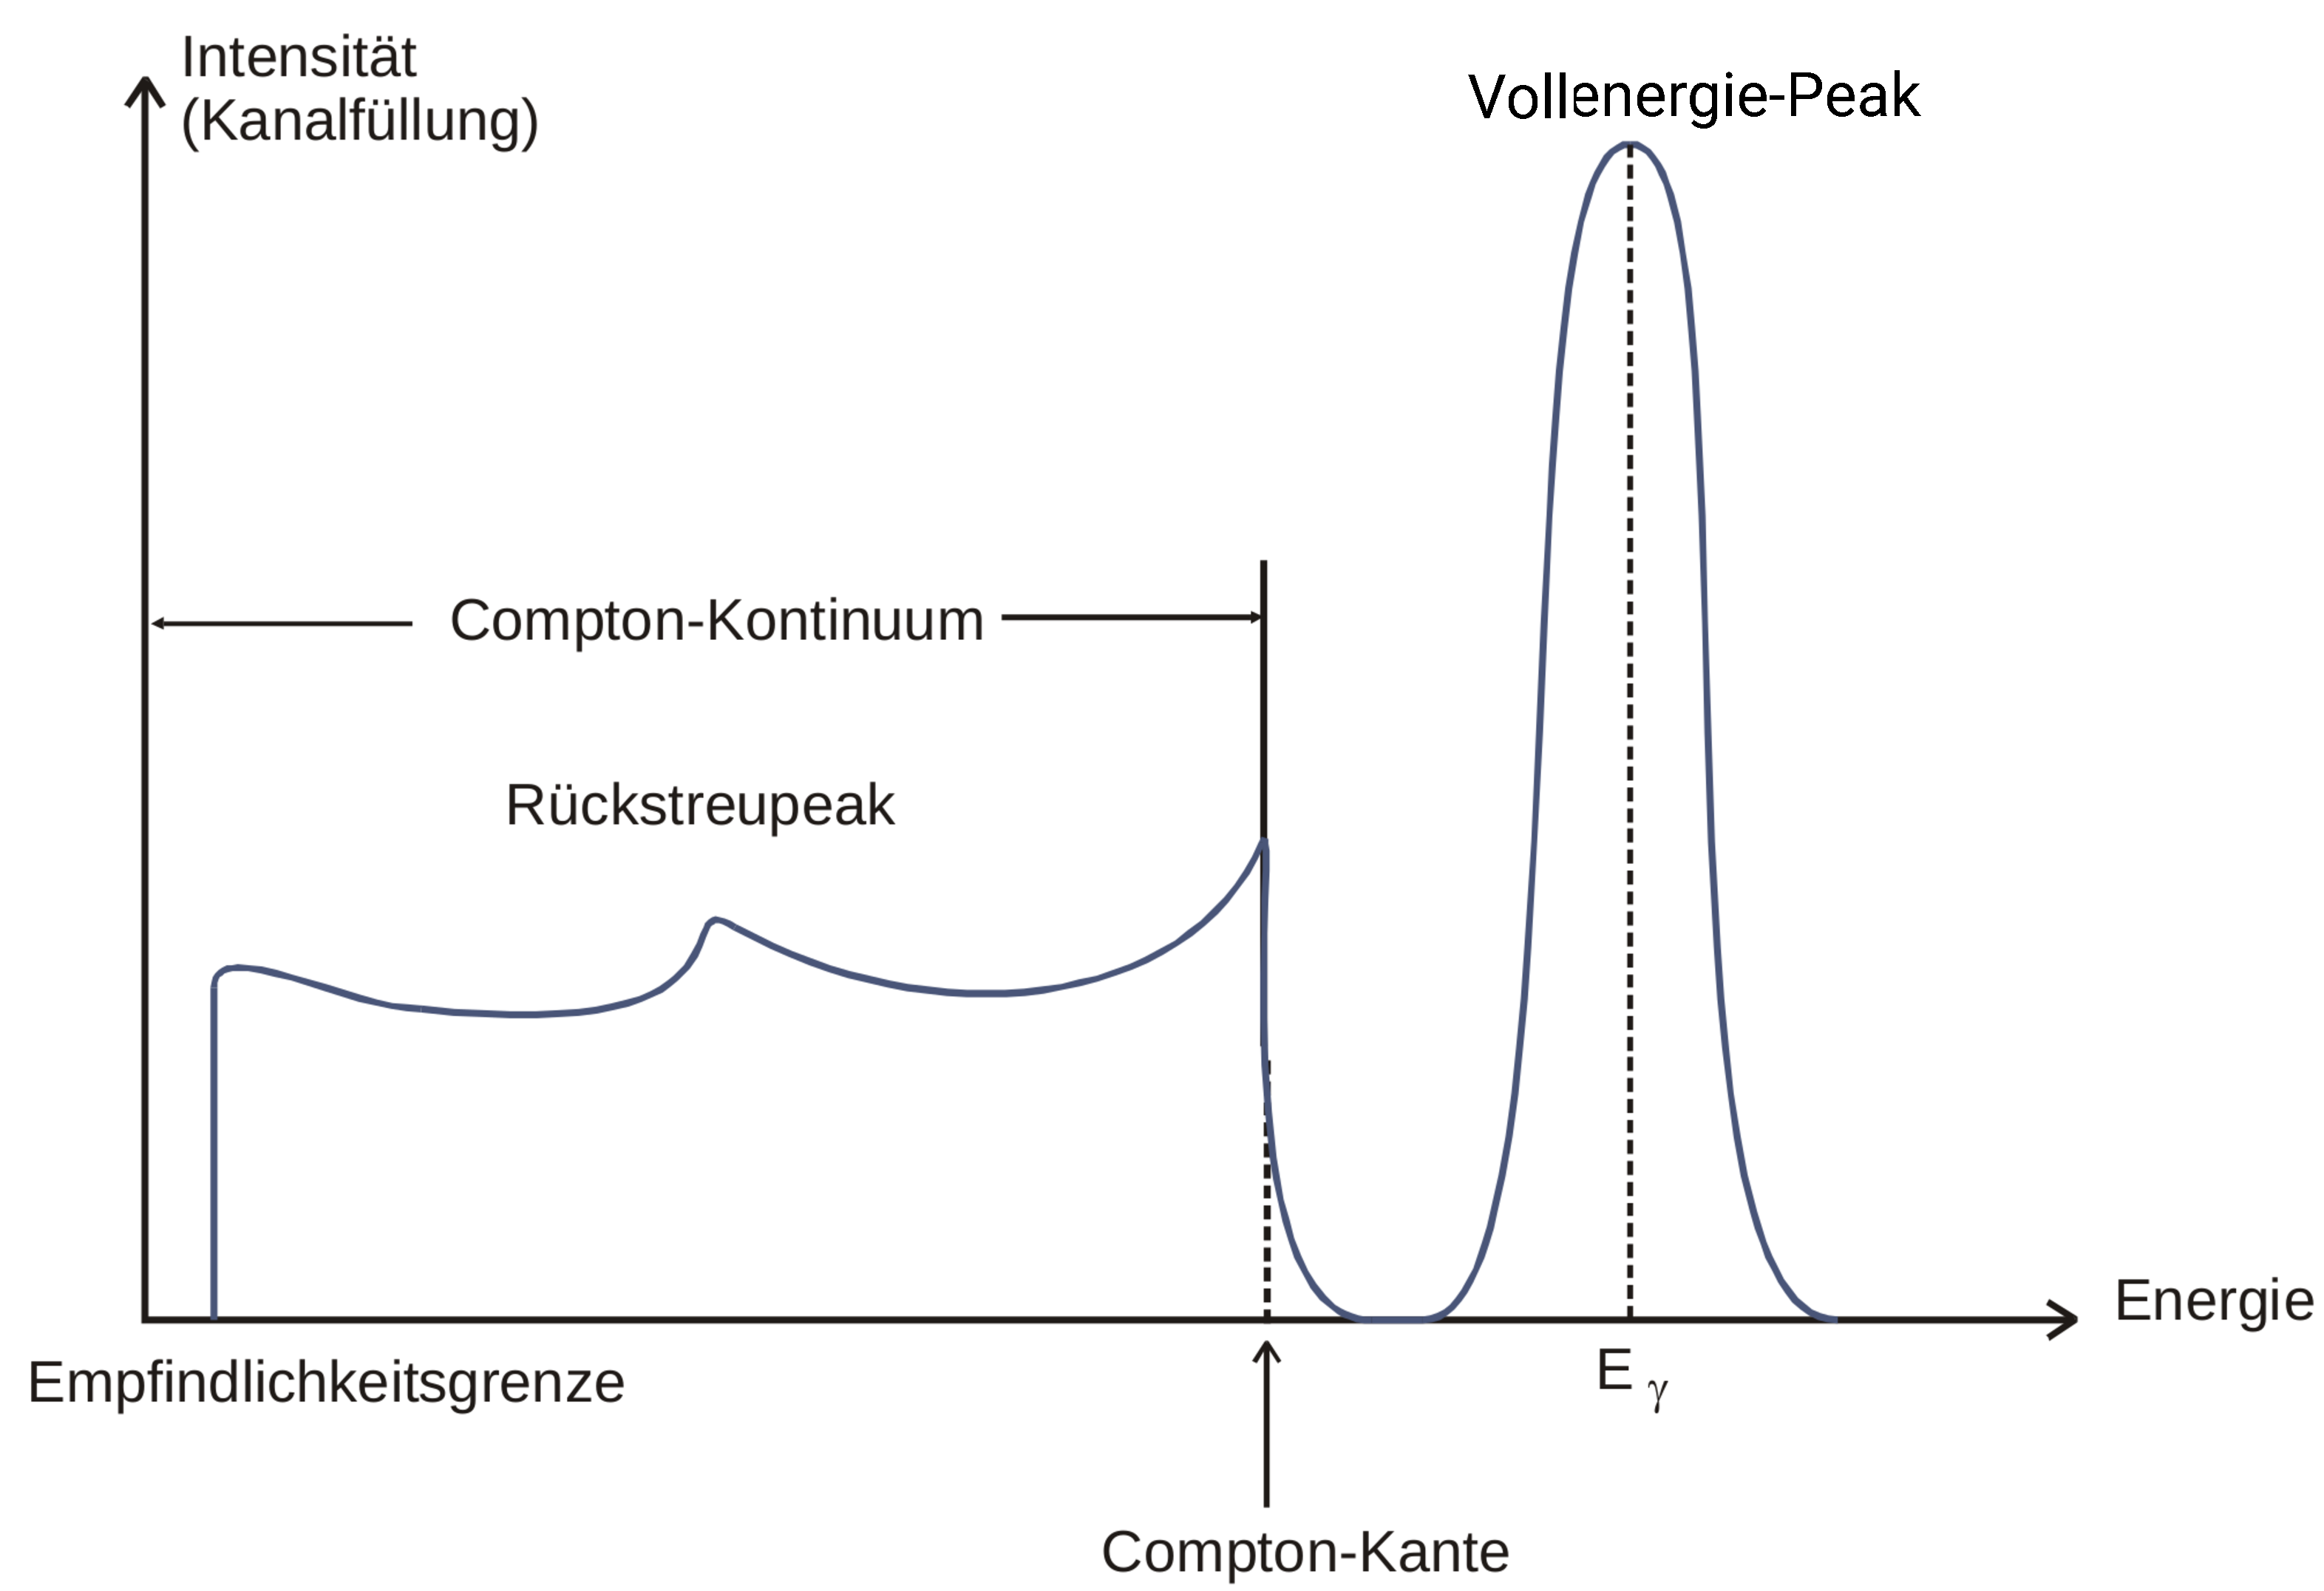
\includegraphics[width = 0.8\textwidth]{pics/example_spectrum.pdf}
\caption{Darstellung eines Energiespektrums, das mit einem Germaniumdetektor aufgenommen wird, nach \cite{anleitungv18}.}
\label{fig: example_spectrum}
\end{figure}

\begin{figure}
\centering
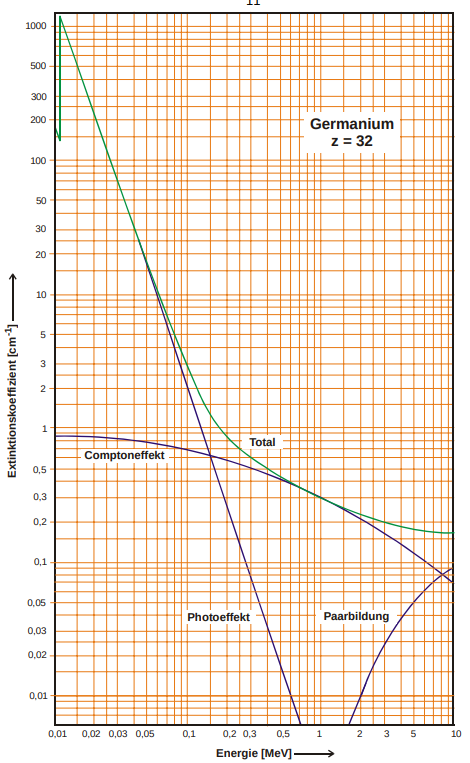
\includegraphics[width = 0.8\textwidth]{pics/extinktionskoeffizient.png}
\caption{Energieabhängigkeit des Extinktionskoeffizienten $\mu$ für Ge getrennt nach den verschiedenen
Wechselwirkungsmechanismen \cite{anleitungv18}.}
\label{fig:extinktionskoeffizient}
\end{figure}
